\documentclass[conference]{IEEEtran}
\IEEEoverridecommandlockouts
% The preceding line is only needed to identify funding in the first footnote. If that is unneeded, please comment it out.
%Template version as of 6/27/2024

\usepackage{cite}
\usepackage{amsmath,amssymb,amsfonts}
\usepackage{algorithmic}
\usepackage{algorithm}
\usepackage{graphicx}
\usepackage{textcomp}
\usepackage{xcolor}
\def\BibTeX{{\rm B\kern-.05em{\sc i\kern-.025em b}\kern-.08em
    T\kern-.1667em\lower.7ex\hbox{E}\kern-.125emX}}
\begin{document}

\title{Deep Reinforcement Learning for Adaptive Non-Primary Channel Access in IEEE 802.11bn}
% Remove funding footnote for now - add back if needed
% \thanks{Identify applicable funding agency here. If none, delete this.}

\author{
\IEEEauthorblockN{Taewon Song}
\IEEEauthorblockA{\textit{Dept. of Internet of Things} \\
\textit{Soonchunhyang University}\\
Asan, Republic of Korea \\
twsong@sch.ac.kr}
}

\maketitle

\begin{abstract}
Efficient spectrum utilization is critical in modern Wi-Fi networks as traditional systems require primary channel occupancy for transmission, limiting efficiency in overlapping BSS (OBSS) environments. IEEE 802.11bn introduces non-primary channel access (NPCA) capability, yet optimal decision strategies remain challenging. This paper presents a deep reinforcement learning approach for adaptive NPCA decision-making using Semi-Markov Decision Process formulation with Deep Q-Network. Simulations across varying network scenarios demonstrate significant throughput improvements over baseline strategies, with contention window index as the most critical decision factor. The learning algorithm exhibits conservative strategies favoring long-term stability, providing insights for next-generation Wi-Fi channel access mechanisms.
\end{abstract}

\begin{IEEEkeywords}
Deep Reinforcement Learning, Non-Primary Channel Access, Wi-Fi Networks, Semi-MDP, OBSS, Channel Access, DQN
\end{IEEEkeywords}

\section{Introduction}

Modern wireless networks face increasing challenges in spectrum efficiency as Wi-Fi deployments become denser and user demands grow. Traditional channel access mechanisms, while effective in simple scenarios, struggle to adapt to dynamic interference patterns and varying network conditions.

IEEE 802.11 systems traditionally require the primary channel to be idle before wide-band transmissions can occur \cite{wei2024non}. This constraint leads to significant spectrum waste when secondary channels remain unused despite primary channel occupancy by overlapping BSS (OBSS) traffic. While IEEE 802.11bn introduces non-primary channel access (NPCA) capability \cite{bellalta2025performance}, existing approaches rely on static heuristics that cannot adapt to dynamic network conditions, leaving a critical gap in intelligent decision-making strategies.

Consider a scenario where a station detects OBSS activity on its primary channel while secondary channels are available. The station must decide whether to wait for primary channel access or switch to NPCA, balancing factors such as transmission duration, channel switching overhead, and future network conditions. Such decisions require adaptive intelligence beyond static rules.

In this paper, we describe an intelligent NPCA decision-making framework that enables stations to learn optimal channel access policies through interaction with dynamic network environments. We formulate this as an online learning problem where stations adapt their behavior based on observed network states and reward feedback.

Our approach employs deep reinforcement learning, specifically a Semi-Markov Decision Process (Semi-MDP) formulation with Deep Q-Network (DQN) \cite{mnih2015human}, to capture temporal dependencies in NPCA decisions. The framework enables stations to learn from experience and adapt to varying OBSS patterns and network densities.

The main contributions of this work are:
\begin{itemize}
\item A Semi-MDP framework for NPCA decision-making that captures temporal dynamics and network state transitions
\item A DQN-based learning algorithm that enables adaptive channel access policies in dynamic environments  
\item Comprehensive performance evaluation demonstrating throughput improvements over baseline strategies
\item Analysis of key decision factors revealing the critical role of contention window index in NPCA decisions
\end{itemize}

The remainder of this paper is organized as follows. Section II reviews related work in NPCA and reinforcement learning applications. Section III presents our system model and problem formulation. Section IV describes the proposed DRL framework. Section V presents simulation results and analysis. Finally, Section VI concludes the paper and discusses future work.

\section{Related Work}

NPCA mechanisms have been extensively studied in the context of spectrum efficiency improvement. Traditional approaches rely on heuristic rules and static thresholds for channel switching decisions \cite{wei2024optimized}. However, these methods fail to adapt to dynamic network conditions and varying traffic patterns.

Reinforcement learning has shown promising results in wireless network optimization \cite{mnih2013playing}. Recent works have applied DRL to various wireless problems, including resource allocation and interference management. Semi-MDP formulations have been particularly effective in capturing temporal dependencies in wireless environments \cite{sutton2018reinforcement}.

Existing NPCA studies focus primarily on theoretical analysis and static optimization. This work addresses the gap by proposing an adaptive learning approach that can respond to real-time network dynamics.

\section{System Model and Problem Formulation}

This section presents the formal mathematical framework for the NPCA decision-making problem, establishing the Semi-MDP~\cite{sutton1999between} formulation that enables intelligent channel access learning.

\subsection{Network Architecture and System Model}

We consider a wireless local area network (WLAN) consisting of two basic service sets (BSSs) operating in the IEEE 802.11bn framework in which Channel 0 with no OBSS interference and Channel 1 with OBSS activity. The stations (STAs) in Channel 1 can opportunistically access the NPCA channel when OBSS activity is detected on the channel.

Each STA in Channel 1 operates according to the enhanced distributed channel access (EDCA) mechanism while maintaining NPCA capability. When OBSS activity is detected on its associated channel during the backoff procedure, the STA will make a strategic decision regarding channel access.

\subsection{State Space Design}

The state space $\mathcal{S}$ captures the essential environmental information required for intelligent NPCA decision-making. At decision epoch $t$, the system state $s_t \in \mathcal{S}$ is represented as a 4-dimensional vector:

\begin{equation}
s_t = \begin{bmatrix} s_t^{(1)} \\ s_t^{(2)} \\ s_t^{(3)} \\ s_t^{(4)} \end{bmatrix} = \begin{bmatrix} T_{obss}(t) \\ T_{radio} \\ T_{tx}(t) \\ CW_{idx}(t) \end{bmatrix}
\label{eq:state_vector}
\end{equation}

where $s_t^{(1)} = T_{obss}(t)$ represents the remaining OBSS occupation time on the primary channel in slots, $s_t^{(2)} = T_{radio}$ denotes the radio transition time required for channel switching in slots, $T_{tx}(t)$ indicates the planned transmission duration for the current PPDU in slots, and $s_t^{(4)} = CW_{idx}(t)$ specifies the current contention window stage index $\in \{0, 1, \ldots, 6\}$.

To ensure numerical stability and bounded input ranges for the neural network, each state component is normalized as

\begin{equation}
\tilde{s}_t^{(i)} = \frac{\min(s_t^{(i)}, C_i)}{C_i}, \quad i \in \{1,2,3,4\}
\label{eq:state_normalization}
\end{equation}
where $C_1 = C_2 = C_3 = 1024$ slots and $C_4 = 8$ represent the normalization caps for each dimension.

State observations occur at specific decision epochs when the STA is in the \texttt{PRIMARY\_BACKOFF} state and detects OBSS activity, regardless of the backoff counter value. This Semi-MDP structure allows decisions at irregular time intervals, capturing the temporal dynamics of wireless channel access.

\subsection{Action Space Formulation}

The action space $\mathcal{A}$ is discrete and binary, representing the fundamental NPCA decision:

\begin{equation}
\mathcal{A} = \{a_0, a_1\} = \{\text{StayPrimary}, \text{GoNPCA}\}
\label{eq:action_space}
\end{equation}

The semantic meaning of each action is:

\begin{itemize}
\item $a_0$ (\texttt{StayPrimary}): The STA maintains its position on the primary channel, transitioning to \texttt{PRIMARY\_FROZEN} state and preserving its current contention window parameters
\item $a_1$ (\texttt{GoNPCA}): The STA switches to the NPCA channel, resetting its contention window index to 0 and generating a new backoff value
\end{itemize}

Once selected, an action defines an ``option'' in the Semi-MDP framework that persists until completion of the transmission attempt. This temporal extension allows the learning algorithm to evaluate long-term consequences of channel access decisions.

\subsection{Reward Function Design}

The reward function implements a delayed reward mechanism that evaluates channel utilization efficiency over complete transmission cycles. Unlike traditional MDP formulations with immediate rewards, our Semi-MDP approach calculates rewards upon option termination.

The episode reward is defined as:

\begin{equation}
R_{episode} = \frac{\sum_{k=1}^{N_{tx}} L_k \cdot \mathbb{I}_{success}(k)}{T_{episode}}
\label{eq:reward_function}
\end{equation}
where $N_{tx}$ is the total number of transmission attempts during the episode, $L_k$ represents the duration (in slots) of the $k$-th transmission attempt, $\mathbb{I}_{success}(k)$ is an indicator function equal to 1 if the $k$-th transmission is successful, 0 otherwise, and $T_{episode}$ is the total episode duration in slots for training stability.

Regarding the success criteria, for primary channel transmissions, a transmission is considered successful if no OBSS interference occurs during the entire transmission duration. For NPCA transmissions, success is defined as the absence of intra-BSS collisions during the transmission. This reward structure encourages the agent to maximize overall spectrum utilization efficiency rather than optimizing for short-term gains, aligning with practical throughput maximization objectives in dense WLAN environments.

\section{Proposed DRL Framework}

This section describes the deep reinforcement learning framework for solving the Semi-MDP formulated NPCA decision problem. We adopt a DQN-based approach with experience replay to handle the temporal dependencies and irregular decision intervals inherent in the Semi-MDP structure.

\subsection{Semi-MDP Learner Architecture}

Our \texttt{SemiMDPLearner} class implements a DQN-based learning algorithm with experience replay and target network stabilization. The neural network architecture consists of three fully connected layers (128, 128, 64 neurons) with ReLU activations and dropout regularization, mapping normalized state observations to Q-values for each action.

The key components include policy network $Q(s,a;\theta)$ for action-value estimation, target network $\hat{Q}(s,a;\hat{\theta})$ for stable learning targets, experience replay memory $\mathcal{D}$ with capacity 10,000 transitions, and Semi-MDP specific transition structure $(s, a, s', R, \tau, done)$, where $\tau$ represents the option duration in slots.

\subsection{Semi-MDP Training Algorithm}

The algorithm initializes the DQN components and iteratively runs episodes of interaction with the environment. At each decision point, it observes the current state, selects an action using an $\epsilon$-greedy policy, and begins a new option. The option continues until termination conditions are met, at which point the accumulated reward and transition are stored in replay memory. Algorithm~\ref{alg:semi_mdp_npca} presents the complete training procedure for the Semi-MDP based NPCA learning system.

\begin{algorithm}[htbp]
\caption{Semi-MDP Training for NPCA Decision Making}
\label{alg:semi_mdp_npca}
\begin{algorithmic}[1]
\STATE Initialize $Q(s,a;\theta)$, target network $\hat{Q}(s,a;\hat{\theta})$, and replay memory $\mathcal{D}$
\FOR{$episode = 1$ to $N_{episodes}$}
    \STATE Reset environment and initialize option variables
    \FOR{$slot = 0$ to $T_{episode}-1$}
        \STATE Advance simulation to next decision point
        \IF{decision point reached}
            \STATE Observe and normalize state $\tilde{s}_t$ 
            \IF{pending option exists}
                \STATE Store transition in $\mathcal{D}$
            \ENDIF
            \STATE Select action $a_t$ using $\epsilon$-greedy with $Q(\tilde{s}_t, a; \theta)$
            \STATE Begin new option: $(s_{option}, a_{option}) \leftarrow (\tilde{s}_t, a_t)$
        \ENDIF
        \STATE Execute step and accumulate option duration $\tau_{option}$
        \IF{option terminates}
            \STATE Calculate option reward $R_{option}$
            \STATE Set pending transition
        \ENDIF
        \IF{$|\mathcal{D}| \geq batch\_size$}
            \STATE Sample mini-batch from $\mathcal{D}$
            \STATE Compute TD targets: \\ 
                \IF{not done}
                    \STATE $y_i = R_i + \gamma^{\tau_i} \max_{a'} \hat{Q}(s'_i, a'; \hat{\theta})$
                \ELSE
                    \STATE $y_i = R_i$
                \ENDIF
            \STATE Update $\theta$ by minimizing \\ 
            \hspace*{\algorithmicindent} $L = \frac{1}{N} \sum_i (y_i - Q(s_i, a_i; \theta))^2$
            \STATE Soft update target network: $\hat{\theta} \leftarrow \tau \theta + (1-\tau) \hat{\theta}$
        \ENDIF
    \ENDFOR
    \STATE Finalize episode with delayed reward \\ 
    \hspace*{\algorithmicindent} based on channel occupancy ratio
\ENDFOR
\RETURN $Q(s,a;\theta)$
\end{algorithmic}
\end{algorithm}

\section{Simulation Results}

\subsection{Experimental Setup}

Simulations are conducted using a time-slotted framework with slot duration of 9 $\mu$s following IEEE 802.11 standards. We evaluate networks with 10 stations per channel, comparing DRL-based NPCA against baseline approaches including primary-only and npca-only strategies.

\subsection{Network Architecture and Hyperparameters}

Our DQN implementation consists of a neural network with three fully connected hidden layers containing 128, 128, and 64 neurons respectively, each followed by ReLU activation functions. Dropout regularization with a rate of 0.1 is applied to prevent overfitting. The input layer receives the 4-dimensional normalized state vector, while the output layer produces Q-values for the two possible actions.

The training process employs experience replay with a memory buffer capacity of 10,000 transitions. Each transition stores the state, action, next state, cumulative reward, option duration ($\tau$), and termination flag. The target network is updated using soft updates with parameter $\tau_{target} = 0.005$.

Key hyperparameters are summarized in Table~\ref{tab:hyperparams}. The learning rate is set to $1 \times 10^{-4}$ with the AdamW optimizer. The discount factor $\gamma = 0.99$ accounts for future rewards, while the epsilon-greedy exploration starts at $\epsilon_{start} = 0.9$ and decays exponentially to $\epsilon_{end} = 0.05$ over 10,000 steps to balance exploration and exploitation.

\begin{table}[htbp]
\caption{DQN Hyperparameters and Network Configuration}
\begin{center}
\begin{tabular}{|l|l|}
\hline
\textbf{Parameter} & \textbf{Value} \\
\hline
\multicolumn{2}{|c|}{\textbf{Network Architecture}} \\
\hline
Hidden layers & [128, 128, 64] neurons \\
Activation function & ReLU \\
Dropout rate & 0.1 \\
Input dimension & 4 (normalized state) \\
Output dimension & 2 (action space) \\
\hline
\multicolumn{2}{|c|}{\textbf{Training Parameters}} \\
\hline
Learning rate ($\alpha$) & $1 \times 10^{-4}$ \\
Discount factor ($\gamma$) & 0.99 \\
Batch size & 128 \\
Replay memory capacity & 10,000 \\
Target network update ($\tau_{target}$) & 0.005 \\
\hline
\multicolumn{2}{|c|}{\textbf{Exploration Strategy}} \\
\hline
$\epsilon_{start}$ & 0.9 \\
$\epsilon_{end}$ & 0.05 \\
$\epsilon_{decay}$ & 10,000 steps \\
\hline
\multicolumn{2}{|c|}{\textbf{Training Episodes}} \\
\hline
Number of episodes & 100 \\
Slots per episode & 1,000 \\
\hline
\end{tabular}
\label{tab:hyperparams}
\end{center}
\end{table}

\subsection{Performance Metrics}

We measure:
\begin{itemize}
\item Throughput: Successful data transmission rate
\item Channel utilization: Ratio of successful channel occupation
\item Fairness: Inter-BSS performance balance
\item Learning convergence: Episode reward progression
\end{itemize}

\subsection{Performance Comparison}

Results demonstrate that the DRL-based approach achieves superior performance compared to static strategies. Across different network scenarios, our method shows significant throughput improvement over baseline approaches including offload-only and local-only strategies. The learning algorithm effectively adapts to varying OBSS patterns and channel conditions.

\subsection{Decision Factor Analysis}

Analysis reveals that contention window index serves as the most critical decision factor, followed by OBSS occupation time. The learned policy exhibits conservative behavior, favoring long-term stability over aggressive short-term gains.

\section{Conclusion and Future Work}

This paper presented a DRL-based approach for adaptive NPCA decision-making in IEEE 802.11bn networks. The Semi-MDP formulation with DQN learning enables stations to intelligently choose between primary and secondary channel access based on dynamic network conditions.

Key findings include the importance of contention window index as a decision factor and the effectiveness of conservative learning strategies. Future work will explore multi-agent learning scenarios and adaptive frame duration optimization based on real-time network conditions.

\begin{table}[htbp]
\caption{Simulation Parameters}
\begin{center}
\begin{tabular}{|l|l|}
\hline
\textbf{Parameter} & \textbf{Value} \\
\hline
Simulation time & 500,000 $\mu$s \\
Slot duration & 9 $\mu$s \\
Number of channels & 2 $\times$ 20 MHz \\
STAs per channel & 2, 6, or 10 \\
Frame duration (Short) & 33 slots (297 $\mu$s) \\
Frame duration (Long) & 165 slots (1485 $\mu$s) \\
OBSS generation rate & 0.05 per slot \\
NPCA switching delay & 5 slots \\
Learning rate & 0.001 \\
Discount factor & 0.99 \\
\hline
\end{tabular}
\label{tab:params}
\end{center}
\end{table}

\begin{figure}[htbp]
\centerline{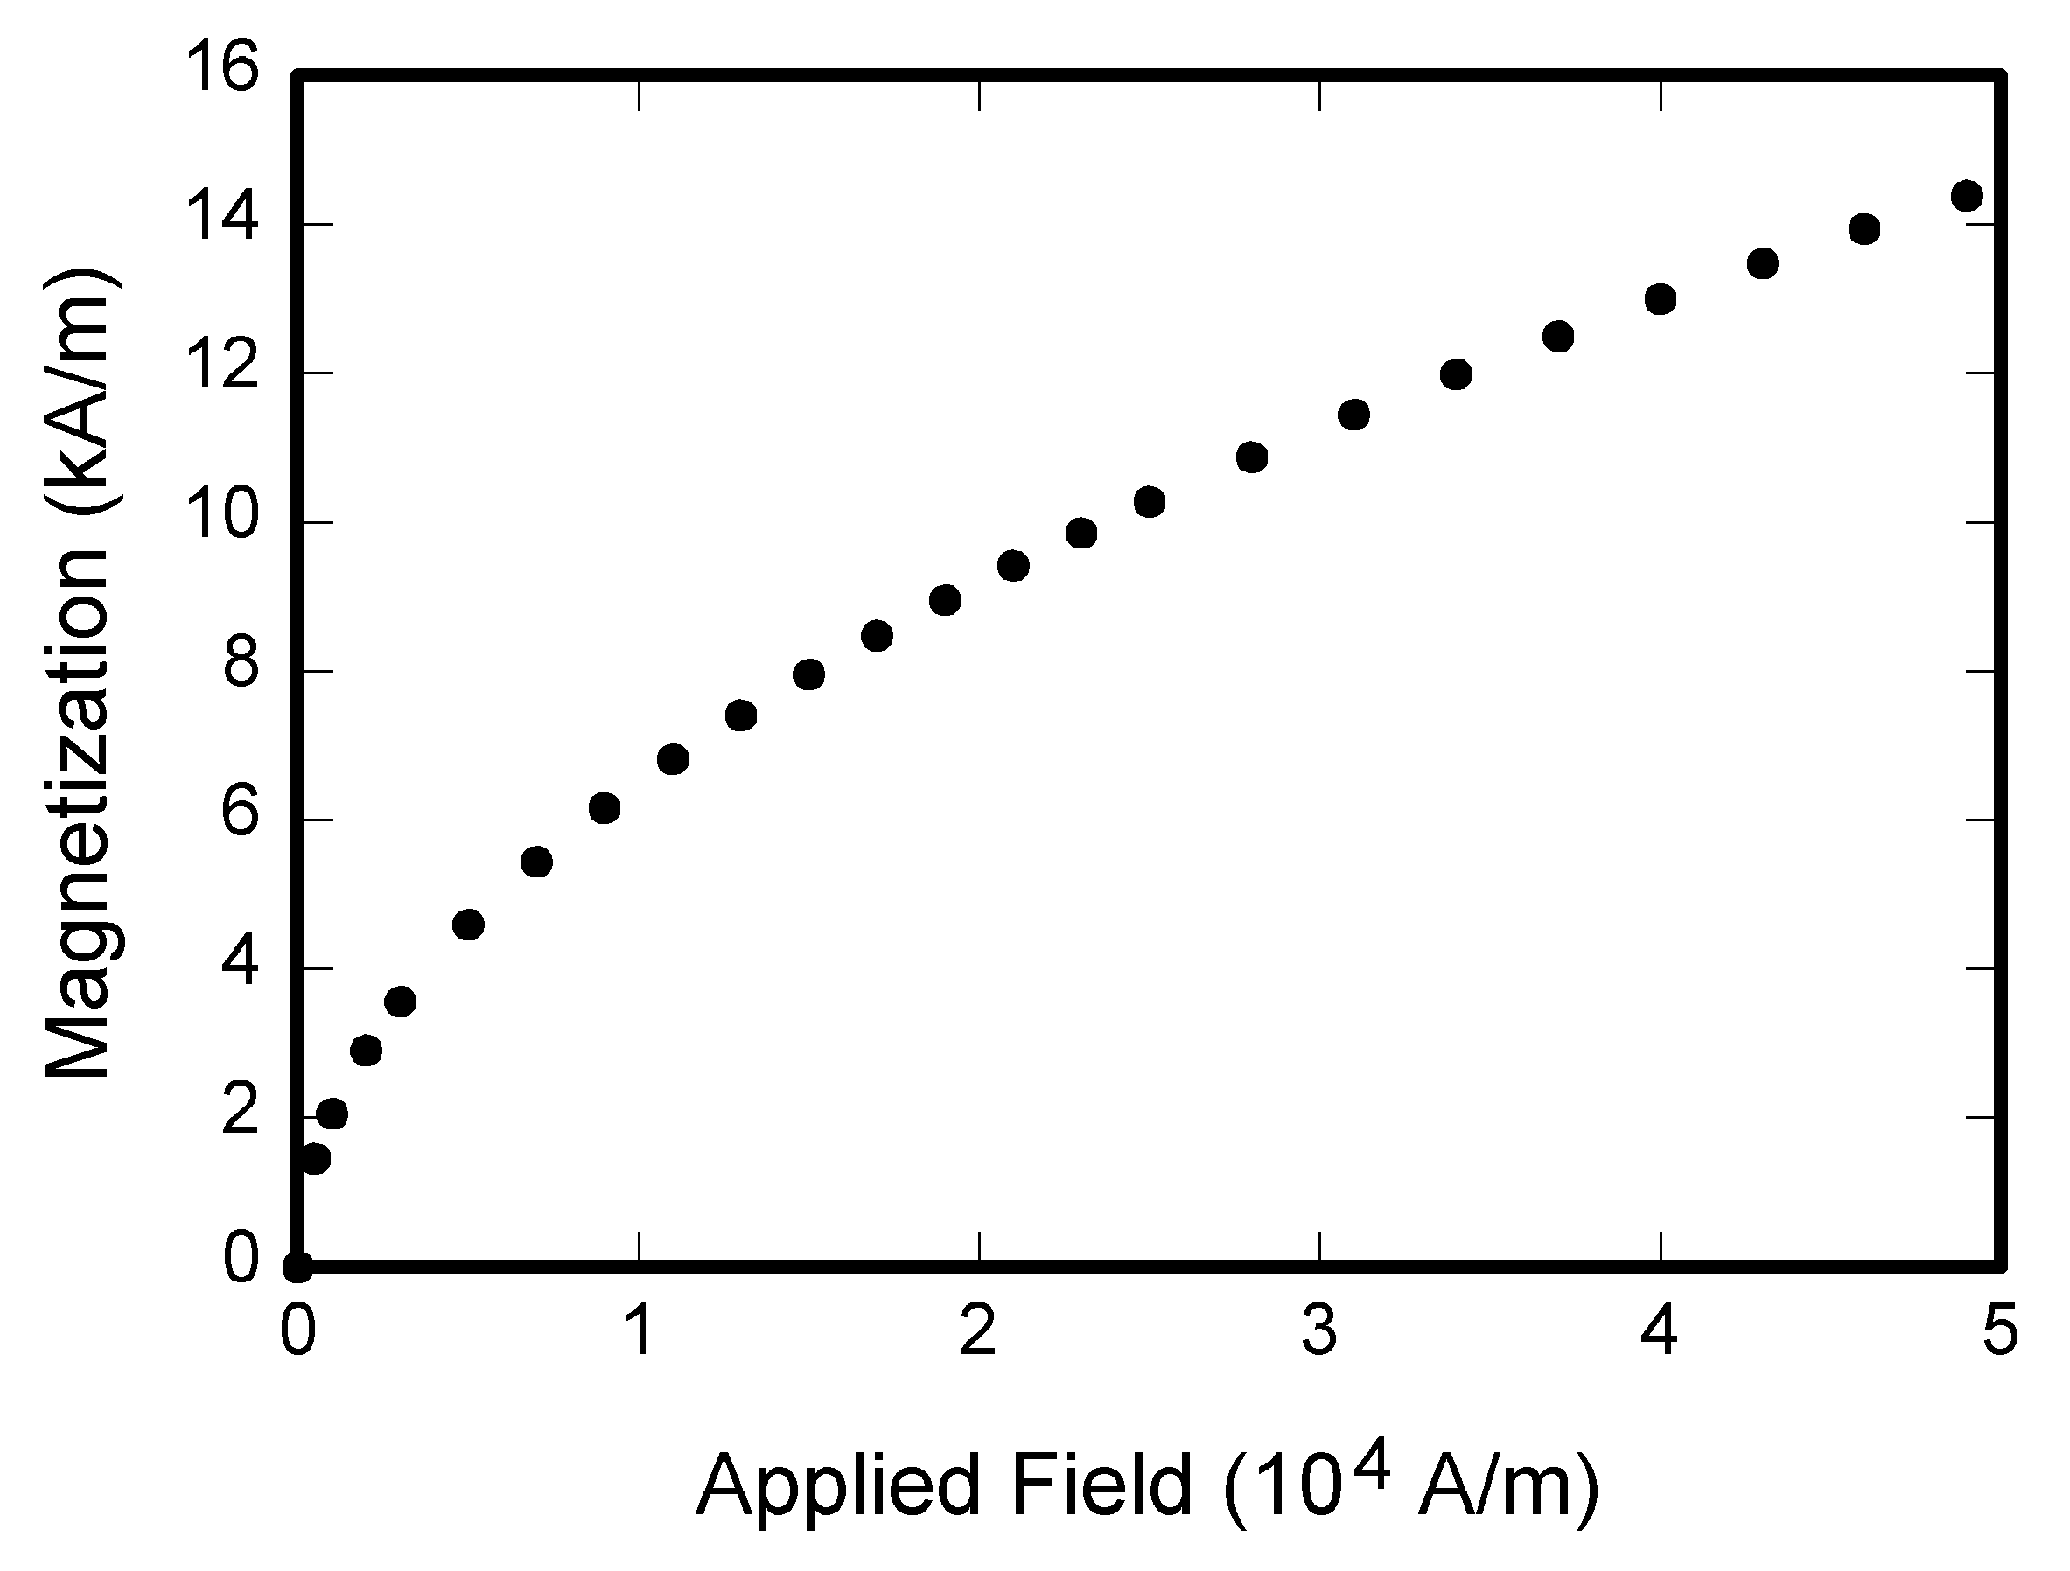
\includegraphics{fig1.png}}
\caption{Training convergence showing episode rewards over time for DRL-based NPCA learning in different network densities.}
\label{fig:training}
\end{figure}

\section*{Acknowledgment}

This research was supported by the MSIT (Ministry of Science and ICT), Korea, under the National Program for Excellence in SW, supervised by the IITP (Institute of Information \& Communications Technology Planning \& Evaluation) in 2025 (2021-0-01399).


\bibliographystyle{IEEEtran}
\bibliography{npca_references}


\end{document}
